% TeXstudio spellcheck 2020-12-10 16:30

\chapter{Háttérismeretek} \label{hatterismeretek}

Ebben a fejezetben összefoglalom a szakdolgozat témájához kapcsolódó háttérismereteket. Bemutatom a modellellenőrzés alapjait (\ref{modellellenorzes}. fejezet), az időzített automaták elméletét és absztrakciós módszereit (\ref{idozitett-automata}. fejezet), az SMT problémákat (\ref{smt}. fejezet), valamint a Theta modellellenőrző keretrendszert (\ref{theta}. fejezet).

\section{Modellellenőrzés} \label{modellellenorzes}

A modellellenőrzés \cite{IntroductionToModelChecking} egy algoritmikus módszer tranzíciós rendszerek dinamikus viselkedésének vizsgálatára. A modellellenőrzéshez (\ref{fig:modell-ell} ábra) alapvetően három dolog szükséges:
\begin{itemize}
    \item \textbf{Formális modell}: Az állapotokat és tranzíciókat tartalmazó véges gráfokkal jól modellezhetők a véges állapotú rendszerek. Esetünkben az időzített automata formalizmussal fogjuk leírni a rendszereket.
    \item \textbf{Formális követelmény}: A modellre vonatkozó általánosabb követelmények megfogalmazhatók pl. temporális logikák \cite{IntroductionToModelChecking} segítségével, ám ezeket szakdolgozatomban nem részletezem. Esetünkben a vezérlési helyek elérhetősége fogja specifikálni a rendszert, ami felírható egy biztonsági követelmény negáltjaként is (a vizsgált invariáns a keresett vezérlési hely elérhetetlensége lesz).
    \item \textbf{Algoritmus}: Szükséges egy olyan algoritmus, amely a modellről eldönti, hogy teljesíti-e a specifikációban foglalt követelményeket.
\end{itemize}

A modellek pontos verifikációja gyakran már kis rendszerek esetében is komoly kihívást jelent, ám teljes bizonyítás nélkül is lehet hasznos a modellellenőrzés hibák felderítésére.

\begin{figure}
    \centering
    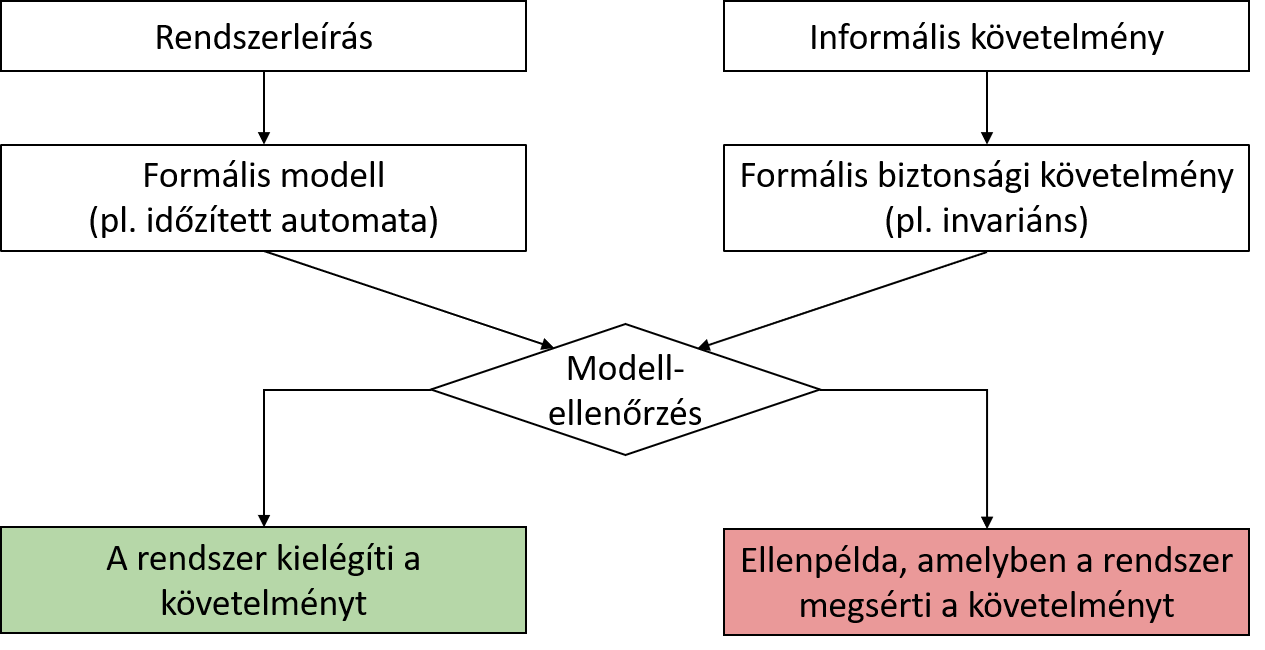
\includegraphics[width=0.85\textwidth, keepaspectratio]{figures/modellell.png}
    \caption{Modellellenőrzés}
    \label{fig:modell-ell}
\end{figure}

%\newpage
A véges állapotú rendszerek formális leírására az egyik legegyszerűbb formalizmus a \emph{Kripke-struktúra} \cite{IntroductionToModelChecking}.

\begin{definition}[Kripke-struktúra]
Egy $K$ \emph{Kripke-struktúra} egy irányított gráf, amelynek csúcsai $A$ atomi tulajdonságok egy-egy részhalmazával vannak címkézve. Formálisan $K = \langle S, R, L \rangle$, ahol
\begin{itemize}
    \item $S$ az állapotok halmaza (az állapottér),
    \item $R \subseteq S \times S$ a tranzíciók halmaza,
    \item $L: S \rightarrow 2^A$ a címkézőfüggvény, amely minden állapothoz az atomi tulajdonságok egy halmazát rendeli.
\end{itemize}
Egy Kripke-struktúra véges, ha $S$ véges.
\end{definition}

Egy $K$ \emph{Kripke-struktúra} $s \in S$ állapotára jelölje $L(s)$ azon atomi tulajdonságok halmazát, amelyek teljesülnek, ha a $K$ rendszer $s$ állapotban van, $A \setminus L(s)$ pedig azon atomi tulajdonságok halmazát, amelyek ugyanekkor nem teljesülnek.

%A \emph{tesztelés} a hibák megtalálásának leggyorsabb és legegyszerűbb módja. Teszteléssel azonban csak megtalálni lehet a hibákat, azok hiányát nem lehet hitelt érdemlően bizonyítani.

\subsection{A modellellenőrzés előnyei és kihívásai}

A modellellenőrzésnek több előnye is van, amely megkülönbözteti más módszerektől, így a teszteléstől is \cite{IntroductionToModelChecking}.
\begin{enumerate}
    \item Egyrészt ez egy algoritmikus módszer, amely automatizálható (szemben a tesztekkel, amelyeket kézzel meg kell írni).
    \item Másrészt a modellellenőrzés a rendszer létrejöttének bármelyik szintjén alkalmazható, vagyis már a tervezés fázisában is ellenőrizhető a rendszer (szemben a teszteléssel, hiszen egy teszt lefuttatása nem lehetséges egy még nem implementált rendszeren).
    \item Harmadrészt a modellellenőrzés konkurens rendszerek vizsgálatára is alkalmas. Ez különösen fontos, hiszen rohamosan terjednek a többprocesszoros rendszerek, a konkurens működés viszont a hibák jelentős hányadát is adja. Ezeket a hibákat viszont teszteléssel nagyon nehéz detektálni, reprodukálni.
\end{enumerate}

A rendszer változóinak számától akár exponenciálisan függhet az állapotok száma (\emph{állapottér-robbanás}), de bizonyos esetekben (pl. valamilyen felső korlát hiánya) akár végtelen is lehet az állapottér. A hatékony, való életbeli rendszereken is alkalmazható modellellenőrzés két kihívást is magában foglal.

\begin{itemize}
    \item Az \emph{algoritmikus kihívás} az algoritmus skálázódására vonatkozik. A nagy állapotterek hatékony kezelése kulcsfontosságú ahhoz, hogy valós méretű rendszereken is alkalmazható legyen az algoritmus.
    \item A \emph{modellezési kihívás} a bonyolult rendszerek formális modelljeinek lekicsinyítését, végessé tételét jelenti pl. absztrakció használatával.
\end{itemize}

A két kihívás természetesen összefügg, a megoldások közösen fejlődnek, hiszen önmagban egyik sem jelent használható módszert.

\subsection{Az állapottér-robbanás kezelése} \label{allapotterRobbanas}

Az állapottér-robbanás kezelése azt jelenti a modellellenőrzés során, hogy megpróbáljuk elkerülni, hogy explicit módon építsük fel és vizsgáljuk a rendszert leíró teljes Kripke-struktúrát (állapotteret). Az ezt célzó módszereket három csoportba sorolhatjuk \cite{IntroductionToModelChecking}.
\begin{itemize}
    \item A \textbf{strukturális módszerek} a rendszer felépítésének (struktúrájának) sajátosságait (pl. szimmetria, rekurzió) használják fel az állapottér kezelésére.
    \item A \textbf{szimbolikus technikák} az állapotok és tranzíciók halmazait valamilyen szimbolikus logikai kifejezéssel írják le (pl. bináris döntési diagram), ezzel tömörítve a teljes rendszer leírását is.
    \item Az \textbf{absztrakció} az eredeti Kripke-struktúra redukálását jelenti egy kisebbre úgy, hogy az is megtartsa az eredetinek bizonyos tulajdonságait.
\end{itemize}

\emph{Absztrakció} használatakor tehát a rendszert leíró $K$ Kripke-struktúrát egy kisebb $\hat{K}$ Kripke-struktúrára (absztrakt modellre) redukáljuk a hatékonyabb feldolgozás érdekében ($\hat{K}$ tehát felülbecslése, elnagyolása $K$-nak). Fontos, hogy az ellenőrizendő követelményünk szempontjából releváns tulajdonságokat nem nagyolhatunk el az absztrakció során, hiszen csak így biztosítható, hogy $\hat{K}$ csak azokat a követelményeket teljesítse, amelyeket $K$ is teljesít.

Jelöljön $\varphi$ egy $K$-n ellenőrizhető követelményt, $K \models \varphi$ pedig azt, ha $K$ teljesíti $\varphi$-t. Formálisan ha $\hat{K}$ szimulálja $K$-t, akkor bármely vizsgált $\varphi$-re ha $\hat{K} \models \varphi$, akkor $K \models \varphi$.

Az \emph{ellenpélda-vezérelt absztrakciófinomítás} \cite{IntroductionToModelChecking} (\ref{fig:cegar} ábra) során iterációnként tovább finomítjuk a $\hat{K}$ absztrakciót, amennyiben ez szükséges.
\begin{itemize}
    \item Ha az absztrakt $\hat{K}$ modell teljesíti a $\varphi$ követelményt, az eredeti $K$ modell is biztosan teljesíti azt (hiszen $\hat{K}$ akkor szimulálja $K$-t (vagyis akkor megfelelő az absztrakció), ha bármely vizsgált $\varphi$-re $\hat{K} \models \varphi \Rightarrow K \models \varphi$).
    \item Ha az absztrakt $\hat{K}$ modell nem teljesíti $\varphi$-t ($\hat{K} \not \models \varphi$), a kapott $\hat{\pi}$ absztrakt ellenpéldát megpróbáljuk konkretizálni.
    \begin{itemize}
        \item Amennyiben ez sikerül, vagyis a $\hat{\pi}$ ellenpélda valódi, az eredeti $K$ rendszer sem teljesíti $\varphi$-t ($K \not \models \varphi$).
        \item Amennyiben a $\hat{\pi}$ ellenpéldát nem sikerül konkretizálni, mert az nem valódi (vagyis csak az absztrakció miatt találhattuk meg), az absztrakt $\hat{K}$-t tovább kell finomítanunk, hogy már ne találhassuk meg benne újra ezt a hamis $\hat{\pi}$ ellenpéldát.
    \end{itemize}
\end{itemize}

\begin{figure}
    \centering
    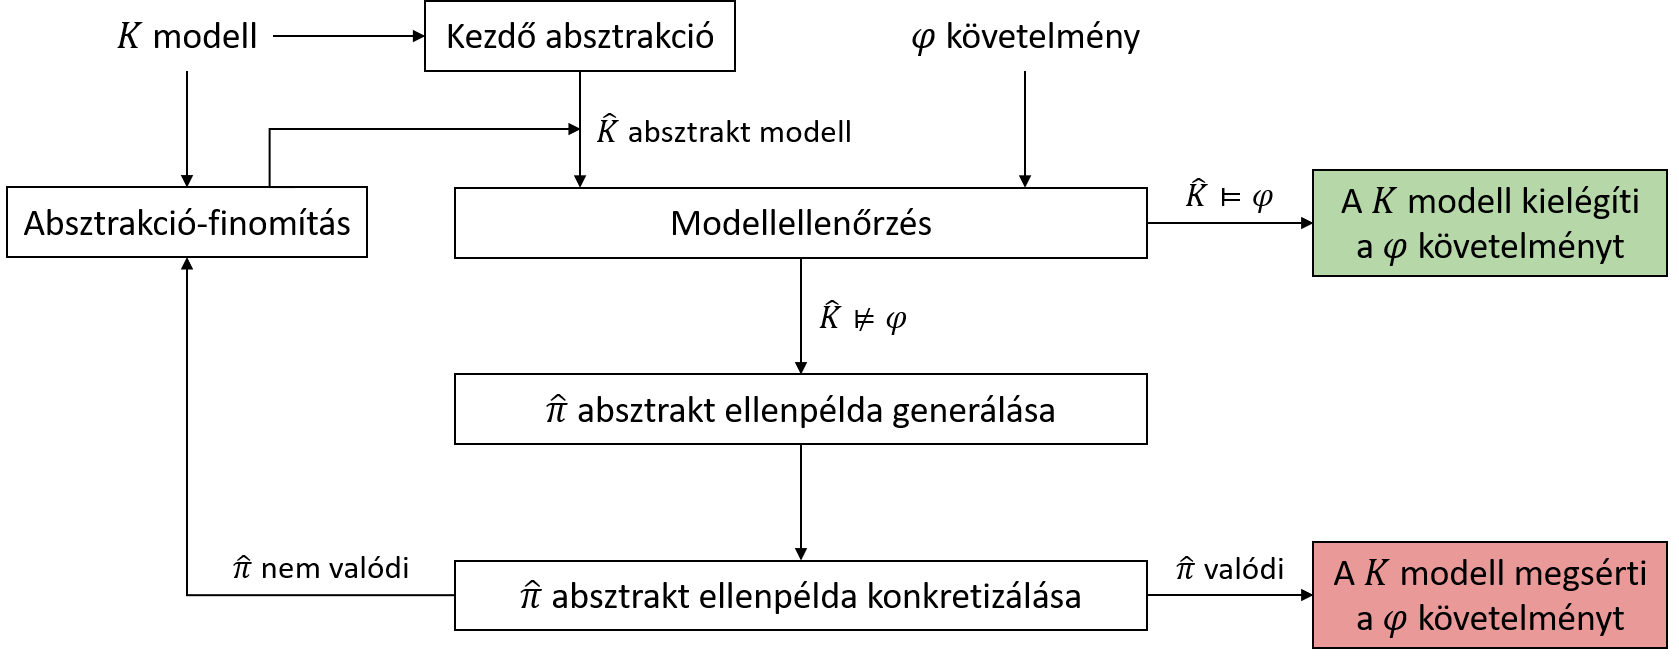
\includegraphics[width=\textwidth, keepaspectratio]{figures/cegar.png}
    \caption{Ellenpélda-vezérelt absztrakciófinomítás}
    \label{fig:cegar}
\end{figure}

\section{Időzített automata} \label{idozitett-automata}

Az időfüggő viselkedésű rendszerek leírására az időzített automata \cite{TimedAutomata} formalizmust alkalmazhatjuk. Az időzített automaták óraváltozókkal kiegészített véges automaták. Az óraváltozók olyan speciális változók, amelyek értéke

\begin{itemize}
    \item valós ($x\in\mathbb{R}$),
    \item 0-ról indul ($x_0=0$),
    \item az automata működése során növekszik (vagyis $x\geq0$),
    \item lenullázható.
\end{itemize}

Jelölje az $x$, $y$ stb. óraváltozók halmazát $\mathcal{C}$, az $a$, $b$ stb. akciók ábécéjét $\Sigma$, az üres akciót $\varepsilon$. Az óraváltozókra ($x \sim n$) vagy azok különbségeire ($x - y \sim n$) megfogalmazhatunk kényszereket (ahol $x$ és $y$ óraváltozók, $\sim$ relációs jel, valamint $n \in \mathbb{N}_0^+$). $\mathcal{B}(\mathcal{C})$-vel jelöljük $\mathcal{C}$-beli óraváltozókra vonatkozó összes lehetséges kényszer halmazát.

\begin{definition}[Időzített automata]
\label{IdőzítettAutomata}
Egy $\mathcal{A}$ \emph{időzített automata} formálisan $\langle L,l_0,T,I\rangle$, ahol
\begin{itemize}
    \item $L$ a vezérlési helyek véges halmaza,
    \item $l_0 \in L$ a kezdő vezérlési hely,
    \item $T \subseteq L \times G \times \Sigma \times 2^\mathcal{C} \times L$ az élek halmaza, ahol $G \subseteq \mathcal{B}(\mathcal{C})$
    \item $I: L \rightarrow 2^{\mathcal{B}(\mathcal{C})}$ a vezérlési helyekhez tartozó invariánsok.
\end{itemize}
\end{definition}

\begin{figure}
    \centering
    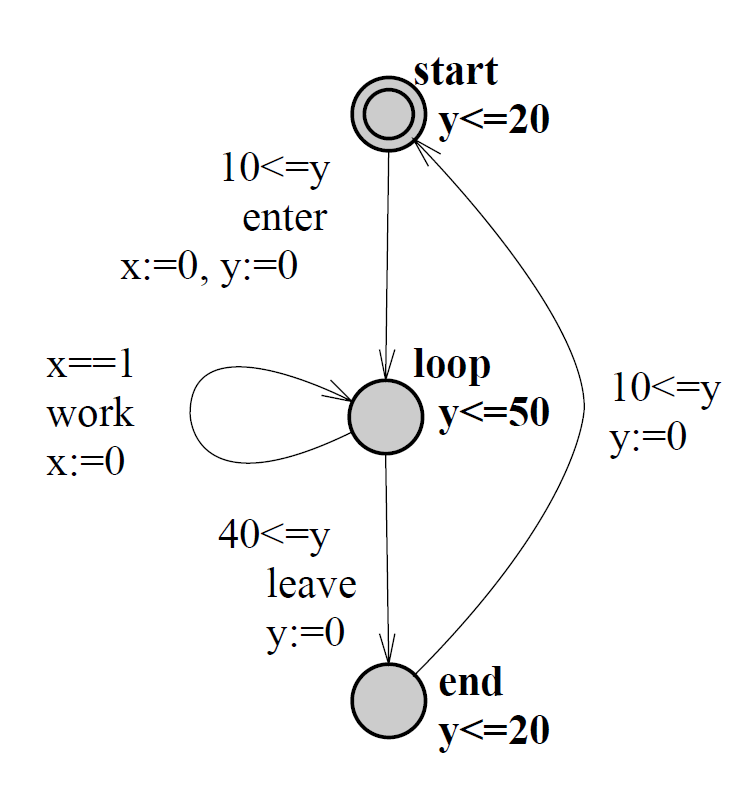
\includegraphics[height=60mm, keepaspectratio]{figures/idozitett-automata-pelda.png}
    \caption{Időzített automata \cite{TimedAutomata}}
    \label{fig:idozitett-automata-pelda}
\end{figure}

\begin{example}[Időzített automata]
A \ref{fig:idozitett-automata-pelda} ábrán látható időzített automata bemeneti ábécéje $\Sigma = \{enter, work, leave\}$, formális leírása $\mathcal{A}^1 = \langle L^1,l_0^1,T^1,I^1 \rangle$, ahol
\begin{itemize}
    \item $L^1 = \{start, loop, end\}$,
    \item $l_0^1 = start$,
    \item $T^1 = 
    \begin{Bmatrix}
    (&start,& \{10 \leq y\},& enter,& \{x, y\},& loop&),\\
    (&loop,& \{x = 1\},& work,& \{x\},& loop&),\\
    (&loop,& \{40 \leq y\},& leave,& \{y\},& end&),\\
    (&end,& \{10 \leq y\},& \varepsilon,& \{y\},& start&)
    \end{Bmatrix}$,
    \item $I^1 = \{ (start \rightarrow \{ y \leq 20 \}), (loop \rightarrow \{ y \leq 50 \}), (end \rightarrow \{ y \leq 20 \}) \}$.
\end{itemize}
\end{example}

Egy $t \in T$ él egy $L$-beli vezérlési helyből egy $L$-beli vezérlési helybe vezet, adott $\mathcal{B}(\mathcal{C})$-beli $G$ őrfeltételek mellett, valamely $\Sigma$-beli akció hatására, a $\mathcal{C}$-beli óraváltozók egy részhalmazának lenullázásával.
Óraváltozókat három módon használhatunk időzített automatákban (ezek mindegyikére mutat példát a \ref{fig:idozitett-automata-pelda} ábra).

\begin{itemize}
    \item 	\textbf{Őrfeltétel élen}: az él csak akkor tüzelhet, ha az őrfeltétel teljesül. A példában a $start$ vezérlési helyről csak akkor léphetünk át a $loop$ vezérlési helyre, ha a $10 \leq y$ feltétel teljesül.
    \item 	\textbf{Lenullázás éllel}: ha az él tüzel, az óraváltozó értéke $0$ lesz. A példában ha az automata az $end$ vezérlési helyről a $start$ vezérlési helyre lép, az $y$ óraváltozó értéke lenullázódik.
    \item 	\textbf{Vezérlési hely invariáns}: az automata csak olyan vezérlési helyen lehet, amelynek az összes invariáns feltétele teljesül. A példában mivel az $end$ vezérlési helyhez az $y \leq 20$ invariáns tartozik, az automatának el kell hagynia az $end$ vezérlési helyet legkésőbb, amikor $y$ értéke $20$ lesz.
\end{itemize}

Jelölje $u$ az óraváltozók egy állását, vagyis egy olyan $\mathcal{C} \rightarrow \mathbb{R}_+$ függvényt, amely értéket rendel minden óraváltozóhoz, $u(x)$ pedig az $x$ óraváltozó értékét az $u$ állásban. Szemantikáját tekintve egy időzített automata egy olyan \emph{Kripke-struktúra}, amelynek állapotai $\langle l, u \rangle$ párok, ahol $l$ egy vezérlési hely, $u$ pedig az óraváltozók egy állása, a címkéző függvény pedig minden állapothoz hozzárendeli az összes ott igaz állítást. A rendszerben kétféle tranzíció (állapotátmenet) lehetséges:
\begin{itemize}
    \item $\langle l, u \rangle \rightarrow \langle l, u + d \rangle$ esetben az automata az $l$ vezérlési helyen várakozik $d$ ideig. Ez értelemszerűen csak akkor lehetséges, ha az $l$ vezérlési helyhez tartozó invariánsokat $u + d$ is kielégíti.
    \item $\langle l, u \rangle \rightarrow \langle l', u' \rangle$ esetben az automata vezérlési helyet vált, $l$-ből $l$'-be lép át. Ez értelemszerűen csak akkor lehetséges, ha van tüzelhető él $l$-ből $l'$-be. Ekkor $u = u'$, kivéve az él által lenullázott óraváltozókat.
\end{itemize}
Egy időzített automata esetében a klasszikus verifikációs probléma az elérhetőség analízis \cite{RealTimeModelChecking}. A megválaszolandó kérdés tehát az, hogy egy $\langle l_0, u_0 \rangle$ kezdőállapotból egy adott $\langle l, u \rangle$ állapot elérhető-e.

Mivel az óraváltozók valós értékkészletű változók, végtelen sok értéket felvehetnek. Ráadásul egy rendszerben nemcsak egy, hanem több óraváltozó is lehet, vagyis egy időzített automata állapottere „többszörösen” végtelen. Adódik tehát az igény ennek az egyszerűsítésére, véges reprezentációjára. Erre több lehetőség is van: a folytonos időt feloszthatjuk régiókra vagy zónákra.

\subsection{Régió}
A valós értékkészletű óraváltozók okozta végtelen állapottér végessé tételének egyik lehetséges módja az idő (az óraváltozók értékkészleteinek) régiókra osztása. Ennél a módszernél azt használjuk ki, hogy az időzített automata működése hogyan függhet az óraváltozók értékeitől. Ha két $u, v$ óraváltozó-állás ugyan különbözik, de ez a különbség az automata működésében nem jelenik meg (és nem is jelenhet meg), tekinthetjük őket azonosnak. Az ezen gondolatmenet alapján azonosnak tekintett állások tartoznak egy régióba, tehát ez a legfinomabb felbontás, amire szükségünk lehet.
\begin{itemize}
    \item Minden $x \in \mathcal{C}$ óraváltozóhoz hozzárendeljük azt a legnagyobb $k(x)$ konstanst, amely rá vonatkozó feltételben szerepel a rendszerben. Az $x$ óraváltozó két $x_i > k(x)$, $x_j > k(x)$ értéke azonosnak tekinthető, hiszen nem lehet két olyan feltétel a rendszerben, amelyre más eredményt adnak.
    
    \item Az óraváltozókra megfogalmazott $x \sim n$ feltételekben $n \in \mathbb{N}_0^+$, vagyis az óraváltozók valós értékét mindig nemnegatív egészekkel hasonlítjuk össze. Az $x$ óraváltozó két $m \in \mathbb{N} < x_i, x_j < m + 1$ értéke tehát ebből a szempontból azonosnak tekinthető, hiszen nem lehet olyan $x \sim n$ feltétel a rendszerben, amelyre más eredményt adnak.
    
    \item Az óraváltozók különbségeire is megfogalmazhatunk kényszereket $x - y \sim n$ alakban, vagyis két $u, v$ óraváltozó-állás nem tekinthető azonosnak, ha van bennük két $x, y$ óra, amelyekre $u(x) \sim u(y)$ és $v(x) \sim v(y)$ $\sim$ relációja nem egyezik meg.
\end{itemize}

Egy példa $\mathcal{C} = \{x, y\}$ két óraváltozós rendszer régiói láthatók a \ref{fig:regiok-pelda} ábrán. A síknegyed vonalak által részben vagy egészben közrezárt területei és \emph{a szakaszok maguk is} külön régiók.

\begin{figure}
    \centering
    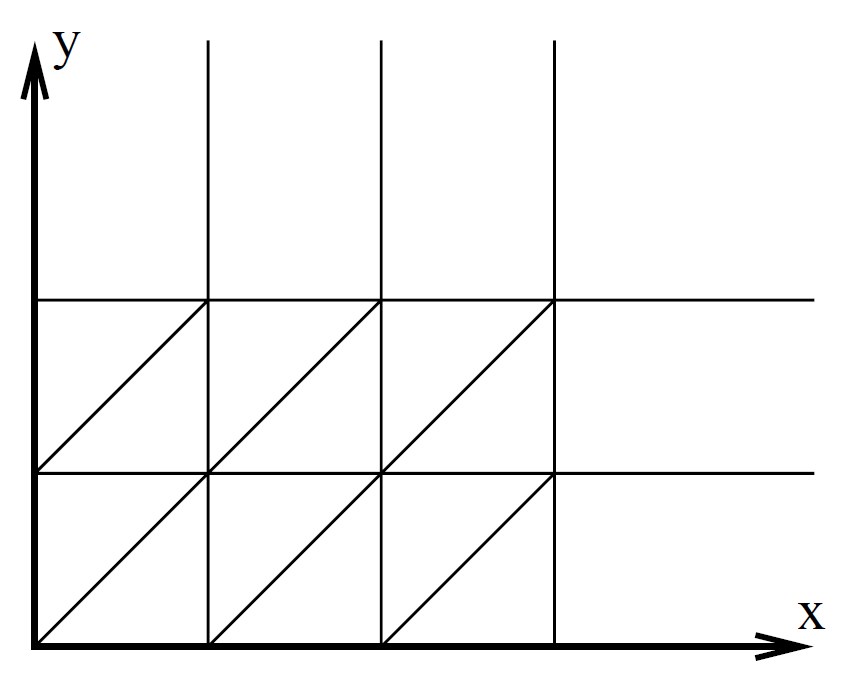
\includegraphics[height=60mm, keepaspectratio]{figures/regiok-pelda.png}
    \caption{Két óraváltozós rendszer régiói \cite{TimedAutomata}}
    \label{fig:regiok-pelda}
\end{figure}

\subsection{Zóna} \label{zona}
Általában nincs szükség a régiók adta granularitásra, ezért a gyakorlatban régiók egy konvex csoportjával dolgozunk: ezt hívjuk zónának.

\begin{definition}[Zóna]
Jelölje $\mathcal{C}$ az óraváltozók halmazát. Zónán a $\mathcal{C}$-beli óraváltozókra vonatkozó $C_i - C_j \sim n$ alakú kényszerek egy (konjunktív) halmazát értjük (ahol $\sim\ \in \{\leq,<,=,>,\geq\}$ és $n \in \mathbb{N}$), de zónának tekinthetjük azt a legtágabb óraváltozóérték-halmazt is, amely kielégíti a kényszerhalmazt.
\end{definition}

A korábban definiált $\langle l, u \rangle$ állapotok helyett bevezetünk $\langle l, \mathcal{Z} \rangle$ szimbolikus állapotokat, ahol $\mathcal{Z}$ egy zóna. A rendszerünk átmenetei ebben az esetben is a korábban leírtak szerint adódnak.

Szimbolikus állapotok alkalmazása esetén értelemszerűen az elérhetőség analízis is szimbolikus állapotokra értendő: a kérdés tehát az, hogy egy $\langle l_0, \mathcal{Z}_0 \rangle$ kezdőállapotból egy adott $\langle l, \mathcal{Z} \rangle$ szimbolikus állapot elérhető-e. Amennyiben $\langle l_f, \mathcal{Z}_f \rangle$-fel jelöljük a rendszer hibaállapotait (vagyis azokat az állapotokat, amelyek bizonyos biztonsági tulajdonságok, követelmények megsértését reprezentálják), a rendszerünk biztonságossága azt jelenti, hogy egyik $\langle l_f, \mathcal{Z}_f \rangle$ állapot sem érhető el.

A \ref{fig:zonagraf-pelda} ábra egy egyszerű időzített automatát és annak zónagráfját mutatja. Ránézésre is látható, hogy a zónagráf az időzített automatánk egy nagyon kompakt (elérhetőség szempontjából azonban teljes) reprezentációja. Hiába vehet fel az $x$ óraváltozó végtelen sok értéket, a zónagráfnak mindösszesen 8 csúcsa van. Látható, hogy a zónagráf csúcsai szimbolikus állapotok, vagyis vezérlési hely és zóna párok.

\begin{figure}
    \centering
    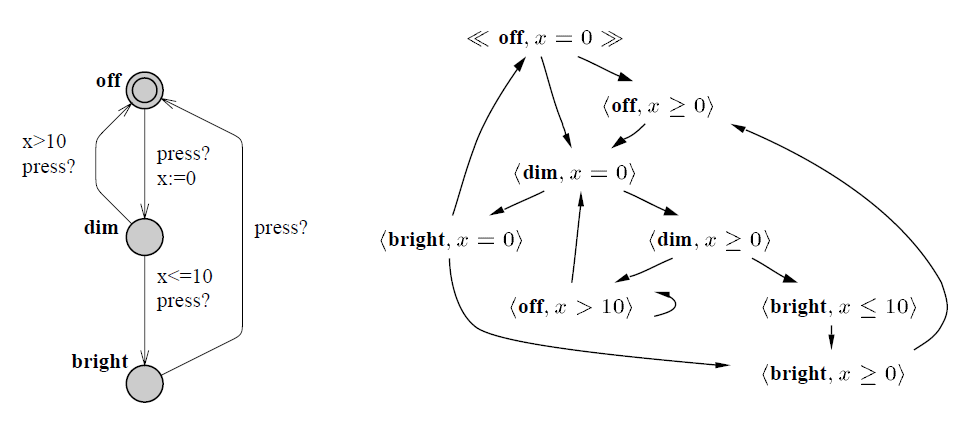
\includegraphics[width=\textwidth, keepaspectratio]{figures/zonagraf-pelda.png}
    \caption{Időzített automata zónagráfja \cite{TimedAutomata}}
    \label{fig:zonagraf-pelda}
\end{figure}

\subsection{Zónák mátrixos ábrázolása}
Az óraváltozókra vonatkozó kényszereknek két alakja lehetséges, ahol $x, y \in \mathcal{C}$, $\sim\ \in \{\leq,<,=,>,\geq\}$ és $n \in \mathbb{N}$. Egy kényszer vonatkozhat egy óraváltozó értékének és egy konstansnak a relációjára ($x \sim n$) vagy két óraváltozó különbségének és egy konstansnak a relációjára ($x-y \sim n$).

A kényszerek kezelése szempontjából kényelmetlen az előbb ismertetett két eltérő alak, ezért bevezetjük a \textbf{0} referenciaórát, amelynek értéke mindig 0. Ennek segítségével az $x \sim n$ alakú kényszerek $x-\textbf{0} \sim n$ alakúra hozhatók, vagyis az összes kényszert leírhatjuk $x-y \sim n$ alakban.

A \textbf{0} referenciaórával kiegészített órahalmazt jelölje $\mathcal{C}_0= \mathcal{C} \cup \{\textbf{0}\}$, az órákat pedig rendezzük sorrendbe, és jelölje az elemeket rendre $C_0,C_1,…,C_n$, ahol $C_0$ a referenciaóra, $C_1,…,C_n$ pedig az eredeti $\mathcal{C}$ órahalmaz.

A $\mathcal{C}_0$-beli óraváltozók különbségeire megfogalmazott kényszereket könnyen reprezentálhatjuk egy $(n+1) \times (n+1)$-es mátrixban, ezt az adatszerkezetet nevezzük \emph{Difference Bound Matrixnak} (DBM). A mátrix $(i,j)$ eleme ($0 \leq i, j \leq |\mathcal{C}|$) reprezentálja a (legszigorúbb) $C_i - C_j \sim n$ kényszert $(n, \sim)$ alakban. Amennyiben egy óraváltozópár különbségére nem vonatkozik kényszer, a mátrix megfelelő mezőjébe $\infty$ kerül.

\begin{example}[Difference Bound Matrix]
Vegyünk például egy rendszert két órával $\mathcal{C} = \{x, y\}$, majd egészítsük ki a \textbf{0} referenciaórával: $\mathcal{C}_0 = \mathcal{C} \cup \{ \textbf{0} \} = \{\textbf{0}, x, y\}$. Az óraváltozóink sorrendje ekkor legyen $C_0 = \textbf{0}, C_1 = x, C_2 = y$. Vegyük azt a $\mathcal{Z}$ zónát, amelyet az $x<20 \wedge y \leq 20 \wedge y-x \leq 10$ kényszerek írnak le. Az $x \sim n$ alakú kényszereket $x-y \sim n$ alakúra hozva a következő kifejezést kapjuk: $\mathcal{Z} = x-\textbf{0}<20 \wedge y-\textbf{0} \leq 20 \wedge y-x \leq 10$.

A $\mathcal{Z}$ zónához tartozó DBM a következő:

\[
M(\mathcal{Z}) = \begin{pmatrix}
(0,\leq) & (0,\leq) & (0,\leq)\\
(20,<) & (0,\leq) & \infty\\
(20,\leq) & (10,\leq) & (0,\leq)
\end{pmatrix}
\]
\end{example}

A $\mathcal{Z}$ zónát leíró $M(\mathcal{Z})$ DBM kapcsán a következő megfigyeléseket tehetjük:
\begin{itemize}
    \item A $\mathcal{Z}$ zónára vonatkozó kényszerek egyértelműen megjelennek az $M(\mathcal{Z})$ mátrixban. Az $x < 20$ ($x - \textbf{0} < 20$) kényszer a mátrix $(1,0)$ elemében $(20,<)$ alakban, az $y \leq 20$ ($y - \textbf{0} \leq 20$) kényszer a mátrix $(2,0)$ elemében $(20,\leq)$ alakban, míg az $y-x \leq 10$ kényszer a mátrix $(2,1)$ elemében $(10,\leq)$ alakban.
    \item A mátrix felső (nulladik) sorában kizárólag $(0,\leq)$ elemek szerepelnek, hiszen itt a $\textbf{0}$ referenciaóra és az óraváltozók negatív különbségeire vonatkozó „kényszerek” szerepelnek. Mivel $\textbf{0}$ értéke mindig 0, az óraváltozók értéke pedig biztosan nemnegatív, $\textbf{0}-C_i = 0-C_i$ értéke biztosan kisebb vagy egyenlő lesz 0-nál.
    \item A mátrix főátlójában is csak $(0,\leq)$ elemek szerepelnek. Ez is értelemszerű, hiszen itt az óraváltozók önmaguktól vett különbségére vonatkozó „kényszerek” állnak ($C_i - C_i \leq 0$).
    \item Mivel a $\mathcal{Z}$ zónában $x-y$-ra nem vonatkozik kényszer, a mátrix hozzá tartozó $(1,2)$ elemében $\infty$ szerepel.
\end{itemize}

A \ref{zona}. fejezetben bevezetett $\langle l, \mathcal{Z} \rangle$ alakú szimbolikus állapotok $\mathcal{Z}$ zónája tehát leírható egy DBM segítségével, vagyis egy szimbolikus állapotot egy vezérlési hely és egy DBM határoznak meg.

\subsection{Absztrakt állapottér-reprezentáció}
Az időzített automaták működésének leírására használhatjuk az Adaptive Simulation Graph (ASG) \cite{spin2018} adatszerkezetet, ez az adatstruktúra az absztrakcióhoz. Az ASG egy olyan gráf, amely az időzített automata (végtelen) lefutásait a (véges) gráfban lévő utakként reprezentálja.
\begin{definition}[Adaptive Simulation Graph]
\label{def:ASG}
Egy $\mathcal{A} = \langle L,l_0,T,I\rangle$ időzített automata $G$ ASG-je formálisan $\langle V, E, v_0, M_v, M_e, \rhd, \psi_Z, \psi_W \rangle$, ahol
\begin{itemize}
    \item $(V, E)$ egy irányított $v_0 \in V$ gyökerű fa gráf,
    \item $M_v: V \rightarrow L$ a csúcscímkézés,
    \item $M_e: E \rightarrow T$ az élcímkézés,
    \item $\rhd \subseteq V \times V$ a fedési reláció,
    \item $\psi_Z, \psi_W: V \rightarrow \{ \mathcal{Z}_i \}$ a csúcsok címkézése zónákkal.
\end{itemize}
\end{definition}

A csúcsok $\psi_Z$ zónacímkézése az állapothoz tartozó pontos zónát jelöli, míg $\psi_W$ ennek egy felülbecslése, absztrakciója. Az elérhetőség vizsgálata közben $\psi_Z$-t valójában nem tároljuk, az algoritmus a kezdetben durva felülbecslést fogja finomítani $\psi_W$-ben annyira, hogy a vizsgált követelmény belátható legyen.

A gráf $v$ csúcsai $\langle l, \mathcal{Z} \rangle$  szimbolikus állapotokat reprezentálnak, ahol $l=M_v(v), \mathcal{Z}=\psi_Z(v)$. A gráf csúcsaira értelmezett fedési reláció azt fejezi ki, hogy az egyik csúcs által reprezentált állapot része egy másik csúcs által reprezentáltnak. Formálisan $v,v' \in V$ csúcsokra $v \rhd v'$ esetén $M_v(v)=M_v(v')$ és $\psi_W(v) \sqsubseteq \psi_W(v')$, vagyis $v'$ fedi $v$-t, ha ugyanaz az állapotcímkéjük, és $v'$ (felülbecsült) zónája tartalmazza $v$ (felülbecsült) zónáját.

%Az ASG generálás legfontosabb kérdése a hatékonyság. Minél kevesebb csúcs kifejtésével szeretnénk megválaszolni az állapotok elérhetőségének kérdését, vagyis végső soron minél kisebb teljes, helyesen címkézett ASG-t szeretnénk kapni. Ez minél több egymást fedő csúcsot jelent, hiszen, ha egy csúcsot lefedünk egy másikkal, már nem kell kifejtenünk.

Absztrakció használatával tehát egy ``durvább`` állapottal reprezentálhatunk több ``finomabb`` állapotot a fedés fogalmára építve. Szükség esetén ezek az absztrakciók finomíthatók a zóna felbontásával, ám erre csak akkor van szükség, ha elérhetőnek tűnik egy olyan állapot, amely valójában nem elérhető. Az elv ugyanaz, mint \aref{allapotterRobbanas}. fejezetben bemutatott absztrakciófinomításnál.
%Az absztrakció jelentőségét az adja, hogy használatával egy tágabb zónával lefedhetünk több kisebb zónájú állapotot (és esetleg néhány olyat is, ami nem elérhető). Vagyis egy állapotfedés annál nagyobb előrelépést jelent, minél tágabb (absztraktabb) a hozzá tartozó zóna. Ebből pedig következik, hogy az absztrakciót csak akkor érdemes finomítanunk, ha muszáj (mert egyébként nem tudnánk lefedni a csúcsot).

Az ASG erejét az adja, hogy egy helyesen címkézett ASG-ből kiolvasható az állapotok elérhetősége. Ez azt jelenti, hogy egy $\mathcal{A}$ időzített automata és annak teljes, helyesen címkézett $G$ ASG-je esetén az alábbi állítások ekvivalensek:
\begin{itemize}
    \item $\mathcal{A}$-nak van $(l_0, \mathcal{Z}_0) \Rightarrow (l_1, \mathcal{Z}_1) \Rightarrow \cdots \Rightarrow (l_n, \mathcal{Z}_n)$ szimbolikus lefutása.
    \item $G$-nek van megfelelő elérhető $v$ csúcsa, hogy $M_v(v) = l_n$.
\end{itemize}

\section{SMT problémák és megoldók} \label{smt}

Az SMT (\emph{Satisfiability Modulo Theories}) \cite{SMT} probléma egy elsőrendű logikai kifejezéseken (feltételeken) értelmezett kielégíthetőségi probléma, vagyis annak az eldöntése, hogy a változóknak (interpretált szimbólumoknak) van-e olyan kiértékelése, hogy az összes feltétel teljesül.

\subsection{Propozicionális logika}
A propozicionális (nulladrendű) logika \cite{SMTTutorial} logikai (bináris) típusú változókon értelmez logikai kifejezéseket.

Egy $\varphi$ nulladrendű logikai formula lehet egy nulladrendű $p$ változó, vagy a $\varphi_0$ és $\varphi_1$ kisebb formulák tagadása ($\neg \varphi_0$), konjunkciója ($\varphi_0 \wedge \varphi_1$), diszjunkciója ($\varphi_0 \vee \varphi_1$), implikációja ($\varphi_0 \Rightarrow \varphi_1$) vagy ekvivalenciája ($\varphi_0 \Leftrightarrow \varphi_1$).

A fenti műveletek igazságtáblái láthatók a \ref{table:logika-ketop-igazsagtabla}. és \ref{table:logika-neg-igazsagtabla}. táblázatban (ahol $\top$ az \emph{igaz}, $\bot$ a \emph{hamis} logikai érték).

\begin{table}[t]
\centering
    \begin{minipage}[b]{0.59\textwidth}%
        \centering
        \begin{tabular}{ c|c||c|c|c|c } 
         $\varphi_0$ & $\varphi_1$ & $\varphi_0 \wedge \varphi_1$ & $\varphi_0 \vee \varphi_1$ & $\varphi_0 \Rightarrow \varphi_1$ &  $\varphi_0 \Leftrightarrow \varphi_1$\\ 
         \hline
         $\top$ & $\top$ & $\top$ & $\top$ & $\top$ & $\top$ \\ 
         $\top$ & $\bot$ & $\bot$ & $\top$ & $\bot$ & $\bot$ \\ 
         $\bot$ & $\top$ & $\bot$ & $\top$ & $\top$ & $\bot$ \\ 
         $\bot$ & $\bot$ & $\bot$ & $\bot$ & $\top$ & $\top$ 
        \end{tabular}
        \subcaption{Kétoperandusú műveletek}
        \label{table:logika-ketop-igazsagtabla}
    \end{minipage}%
    \hspace{0.01\textwidth}%
    \begin{minipage}[b]{0.3\textwidth}%
        \centering
        \begin{tabular}{ c||c } 
         $\varphi_0$ & $\neg \varphi_0$  \\ 
         \hline
         $\top$ & $\bot$ \\ 
         $\bot$ & $\top$ \\
         \multicolumn{2}{c}{} \\
         \multicolumn{2}{c}{} \\
        \end{tabular}
        \subcaption{Tagadás (negáció)}
        \label{table:logika-neg-igazsagtabla}
    \end{minipage}%
    \caption{A nulladrendű logika műveleteinek igazságtáblái}
    \label{tab:my_label}
\end{table}

Egy $\varphi$ formula $M$ kiértékelése minden $\varphi$-beli változóhoz egy $\{\top,\bot\}$-beli igazságértéket rendel. Egy adott $\varphi$ formula \emph{kielégíthető}, ha van olyan $M$ kiértékelése, hogy $M \models \varphi$ a fenti igazságtáblák alapján. $\varphi$ \emph{érvényes}, ha minden $M$ kiértékelésre $M \models \varphi$. Minden nulladrendű formula vagy érvényes vagy a tagadása kielégíthető.

Egy \emph{literál} egy nulladrendű $p$ változó vagy annak $\neg p$ tagadása. Egy $p$ literál tagadása $\neg p$, $\neg p$ tagadása pedig $p$. Egy formula egy \emph{klóz}, ha literálok diszjunkciója $l_1 \vee \dots \vee l_n$ alakban $l_i$ literálokra, ahol $1 \leq i \leq n$. Egy formula \emph{konjunktív normálformában} (CNF) van, ha klózok konjunkciója $\Gamma_1 \wedge \dots \wedge \Gamma_m$ alakban $\Gamma_i$ klózokra, ahol $1 \leq i \leq m$.

\subsection{Elsőrendű logika}
Egy elsőrendű logikai szignatúra \cite{SMTTutorial} definiálásakor feltételezünk három megszámlálható halmazt: \emph{változókat} ($X$), \emph{függvényjeleket} ($\mathcal{F}$) és \emph{predikátumjeleket} ($\mathcal{P}$).

Egy $\Sigma$ elsőrendű logikai \emph{szignatúra} egy részleges $\mathcal{F} \cup \mathcal{P} \rightarrow \mathbb{N}$ hozzárendelés, amely a függvényjelekhez és predikátumjelekhez egy természetes számot rendel az \emph{aritásuknak} megfelelően.

Egy $\tau$ \emph{$\Sigma$-term}
\[
\tau := x \mid f(\tau_1,\dots,\tau_n)
\]
alakú, ahol $x \in X$, $f \in \mathcal{F}$ és $\Sigma(f) = n$. Például, ha $\Sigma(f) = 2$ és $\Sigma(g) = 1$, akkor $f(x,g(x))$ egy $\Sigma$-term.

Egy $\psi$ \emph{$\Sigma$-formula}
\[
\psi := p(\tau_1,\dots,\tau_n) \mid \tau_0 = \tau_1 \mid \neg \psi_0 \mid \psi_0 \vee \psi_1 \mid \psi_0 \wedge \psi_1 \mid (\exists x: \psi_0) \mid (\forall x: \psi_0)
\]
alakú, ahol $p \in \mathcal{P}$, $\Sigma(p) = n$ és $\tau_i$ egy $\Sigma$-term, ahol $1 \leq i \leq n$. Például, ha egy $<$ predikátumjelre $\Sigma(<) = 2$, akkor $(\forall x: (\exists y: x < y))$ egy $\Sigma$-formula.

Egy változó szabad $\psi$-ben, ha nem szerepel $\forall$ vagy $\exists$ kvantor után. Egy $\psi$ formula szabad változóit $vars(\psi)$-vel jelöljük. A \emph{zárt kifejezés} olyan formula, amelynek nincs szabad változója, vagyis $\psi$ zárt kifejezés, ha $vars(\psi) = \emptyset$.

Egy $M$ $\Sigma$-struktúra tartalmaz egy nem-üres $|M|$ domént, ahol:
\begin{itemize}
    \item minden $x \in X$-re $M(x) \in |M|$, vagyis $x$ értékei $|M|$-ből kerülnek ki;
    \item minden $f \in \mathcal{F}$-re, ahol $\Sigma(f) = n$, $M(f)$ egy leképezés $|M|^n$-ről $|M|$-re, vagyis $n$ db argumentumhoz rendel egy értéket; 
    \item minden $p \in \mathcal{P}$-re, ahol $\Sigma(p) = n$, $M(p)$ az $|M|^n$ egy részhalmaza, vagyis azok az $n$-esek, amikre a predikátum igaz.
\end{itemize}

Egy adott $a$ $\Sigma$-term interpretációja egy $M$ $\Sigma$-struktúrában $M\llbracket a \rrbracket = M(a)$ és $M\llbracket f(a_1,\dots,a_n) \rrbracket = M(f)(M\llbracket a_1\rrbracket,\dots,M\llbracket a_n \rrbracket)$.

Egy $\psi$ $\Sigma$-formulára és egy $M$ $\Sigma$-struktúrára az $M \models \psi$ kielégítés a következőképpen definiálható:

\begin{align*}
    M \models a = b &\iff M \llbracket a \rrbracket = M \llbracket b \rrbracket \\
    M \models p(a_1,\dots,a_n) &\iff (M \llbracket a_1 \rrbracket,\dots,M \llbracket a_n \rrbracket) \in M(p) \\
    M \models \neg \psi &\iff M \not \models \psi \\
    M \models \psi_0 \vee \psi_1 &\iff M \models \psi_0 \text{ vagy } M \models \psi_1 \\
    M \models \psi_0 \wedge \psi_1 &\iff M \models \psi_0 \text{ és } M \models \psi_1 \\
    M \models (\forall x: \psi) &\iff M\{x \mapsto \textbf{a}\} \models \psi, \text{ minden } \textbf{a} \in |M|\text{-re} \\
    M \models (\exists x: \psi) &\iff M\{x \mapsto \textbf{a}\} \models \psi, \text{ valamely } \textbf{a} \in |M|\text{-re}
\end{align*}

Egy elsőrendű $\psi$ $\Sigma$-formula \emph{kielégíthető}, ha van olyan $M$ $\Sigma$-struktúra, amelyre $M \models \psi$; továbbá \emph{érvényes}, ha minden $M$ $\Sigma$-struktúrára $M \models \psi$. Minden $\Sigma$-zártkifejezés vagy kielégíthető vagy a tagadása érvényes.

\subsection{SMT probléma}
Egy SMT probléma feltételei többek között lehetnek a változókra vonatkozó lineáris egyenlőtlenségek, mint pl. $x + 2y - 3z \leq 19$.

Az SMT probléma felfogható a SAT (\emph{Boolean satisfiability problem}) probléma kiterjesztéseként is, hiszen míg SAT-esetben bináris változókra ($x \in \{0, 1\}$) szorítkozunk, SMT esetben a változók nem-bináris, hanem pl. racionális ($x \in \mathbb{Q}$) értékkészletűek. A nem-bináris változókra vonatkozó logikai kifejezések viszont ugyanúgy bináris értékűek (vagy teljesülnek vagy nem).

\subsection{SMT megoldók} \label{smt-megoldok}

Az SMT megoldók (solverek) működésük szerint kétfélék lehetnek.
\begin{itemize}
    \item \textbf{Mohó} (\emph{eager}) módszer: Az SMT problémát lefordítják SAT problémára (vagyis a magasabb szintű problémát lefordítják alacsonyabb, bináris szintre), majd átadják egy SAT megoldónak. Ennek előnye, hogy a már létező SAT solverek használhatók SMT problémákra is, hátránya ugyanakkor, hogy a magasabb szintű szemantika elvesztésével a SAT megoldónak gyakran a szükségesnél nehezebb feladatot kell megoldania. (Pl. ha egy 32 bites egész számot 32 egybites bináris változóra fordít le a mohó SMT solver, akkor egy $x+y = y+x$ egyenlőség triviális voltát már nem olyan könnyű észrevennie.)
    \item \textbf{Lusta} (\emph{lazy}) módszer: Ez az előbbi felismerés vezetett el a lusta SMT megoldókhoz. Ezek csak integrálják a SAT megoldók bináris logikáját az elméletspecifikus megoldókba (ún. T-megoldókba), amelyek az adott elméleten (pl. egész számok) képesek dolgozni.
\end{itemize}

Az SMT megoldóknak nagy jelentőségük van a számítástudományban, ugyanis számos fontos probléma (így a modellellenőrzés is) visszavezethető logikai kifejezések kielégíthetőségének vizsgálatára.

Az SMT megoldó programoktól a következő funkcionalitást várjuk el:
\begin{itemize}
    \item \textsc{Hozzáadás}: Egy új kényszer hozzáadása a meglévőkhöz.
    \item \textsc{Push}: Az aktuális kényszerkonfiguráció mentése a kényszerkonfigurációk közé.
    \item \textsc{Pop}: A legutóbb mentett kényszerkonfiguráció betöltése, és törlése a kényszerkonfigurációk közül.
    \item \textsc{Megoldás}: Az aktuális kényszerek megoldása.
\end{itemize}

A \textsc{Push} és \textsc{Pop} egy \emph{stack}-szerű (LIFO: last in, first out) működést biztosít a mentett kényszerkonfigurációkhoz (visszaállítási pontokhoz).

Egy széleskörűen használt SMT megoldó a Microsoft Research által C++ nyelven fejlesztett, nyílt forráskódú \emph{Z3 Theorem Prover}.\footnote{\url{https://github.com/Z3Prover/z3/wiki}} A Z3 többek között C, C++, C\#, Java, és Python nyelvű API-kon keresztül is elérhető.

\section{Theta} \label{theta}
A Theta \cite{Theta} egy generikus, moduláris, konfigurálható modellellenőrző keretrendszer, amelyet a Budapesti Műszaki és Gazdaságtudományi Egyetem Méréstechnika és Információs Rendszerek Tanszékén fejlesztenek. Absztrakciófinomítás-alapú algoritmusok fejlesztését és használatát teszi lehetővé különböző formalizmusok elérhetőségi analízisének megoldására.

\subsection{Felépítés} \label{Theta:felepites}

A Theta fő előnye a felépítése (\ref{fig:theta} ábra), amely lehetővé teszi különböző absztrakt domének, interpreterek és absztrakciófinomítási módszerek kombinálását különböző formalizmusú modelleken.

\begin{figure}
    \centering
    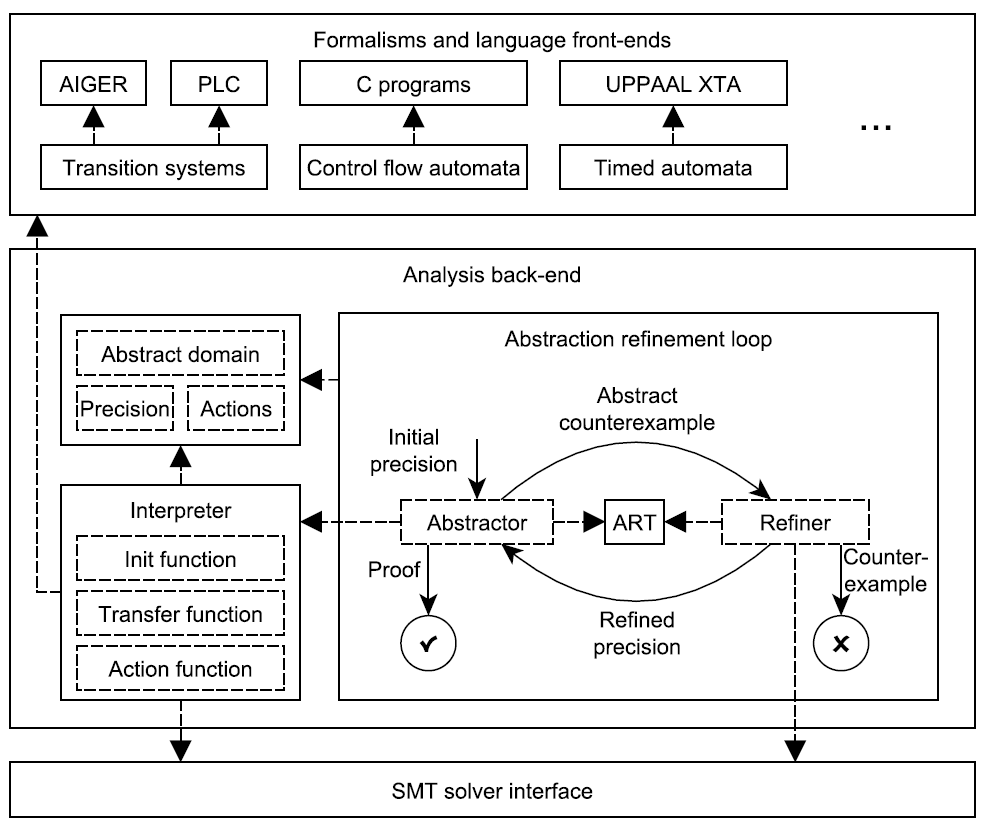
\includegraphics[width=0.9\textwidth, keepaspectratio]{figures/theta.png}
    \caption{A Theta keretrendszer felépítése \cite{Theta}}
    \label{fig:theta}
\end{figure}

A Theta felépítését tekintve három fő részre osztható: a formalizmusok és nyelvi front-endek (\emph{formalisms and language front-ends}), az analízis back-end (\emph{analysis back-end}) és az SMT megoldó interfész (\emph{SMT solver interface}).

A Theta egyik célja, hogy különböző formalizmusokat is támogasson. Az alacsony szintű matematikai reprezentációkhoz (elsőrendű logika kifejezések, gráfalapú leírások) magasabb szintű nyelvi front-endek is tartoznak, amelyek parszerek és interpreterek segítségével képződnek le alacsonyabb szintre. A támogatott formalizmusok jelenleg tranzíciós rendszerek (PLC vagy AIGER nyelvről), control flow automaták (C programnyelvből) és időzített automaták (UPPAAL XTA nyelvből). A moduláris felépítésből adódóan azonban a támogatott nyelvek és formalizmusok tovább bővíthetők, a dolgozat írásakor végéhez közeledik az XSTS és XCFA formalizmusok fejlesztése.

Az analízis back-end három fő részből áll: az absztrakt doménből (\emph{abstract domain}), a formalizmusfüggő interpreterből (\emph{interpreter}) és az absztrakciófinomítási ciklusból (\emph{abstraction refinement loop}).

Az analízis alapja az absztrakt domén, az absztrakt állapotok halmazával (valamint az alsó elemmel és egy állapotokon értelmezett részleges rendezéssel). Egy adott analízis pontosságát (\emph{precision}) a modellből nyilvántartott információk halmaza adja. Továbbá az adott formalizmus meghatározza az akciók halmazát (\emph{actions}).

Az interpreter definiálja az absztrakt állapotokon és akciókon értelmezett működési szemantikát, adott pontossággal. Az absztrakt kezdőállapotokat az inicializáló függvény (\emph{init function}) adja meg, míg egy absztrakt állapotot adott akcióra követő utód állapot az átviteli függvénnyel (\emph{transfer function}) számítható ki. Az akció függvény (\emph{action function}) az elérhető akciókat rendeli egy absztrakt állapothoz.

Az elérhetőség analízist az absztrakciófinomítási ciklus végzi el, melynek központi adatstruktúrája az absztrakt elérhetőségi fa (\emph{ART: abstract reachability tree}), melynek csúcsai absztrakt állapotokkal (amik elérhető állapotok absztrakt felülbecslései), élei pedig akciókkal címkézettek. A \ref{def:ASG}. definícióban bevezetett Adaptive Simulation Graph is egy ART az XTA formalizmushoz. Az ART-t a ciklus két fő eleme módosítja: az absztraháló (\emph{abstractor}) és a finomító (\emph{refiner}).

Az interpreter segítségével a kezdeti pontosság (\emph{initial precision}) és az adott absztrakciós stratégia (algoritmus) alapján az absztraháló előállítja a kezdeti ART-t. Ha az ART-ben nincs ellenpélda, az bizonyítja (\emph{proof}) a modell helyességét (biztonságosságát). Ellenkező esetben (vagyis ha az absztraháló az ART-ben talál absztrakt ellenpéldát) a finomító ellenőrzi az absztrakt ellenpélda elérhetőségét. Amennyiben elérhető, vagyis valódi ellenpélda, a modell hibás (nem biztonságos), egyébként pedig a finomító úgy finomítja az ART absztrakcióját, hogy ezt a valójában nem elérhető ellenpéldát már ne tartalmazza (lásd \ref{modellellenorzes}. fejezet).

Az SMT megoldó interfész egy általános interfész, amely támogatja többek között az inkrementális megoldást is (\aref{smt-megoldok}. fejezetben bemutatott \textsc{Push} és \textsc{Pop} műveletek). Ezt az interfészt használják az analízis komponensek az állapotok részleges rendezéséhez és az átviteli függvényhez, de a finomító is használhatja egy absztrakt ellenpélda elérhetőségének vizsgálatához vagy az absztrakció finomításához, Az interfészt többek között a jelenleg elsődlegesen használt Z3 SMT megoldó implementálja, de könnyen bővíthető további megoldókkal.

\subsection{Megvalósítás}

A Theta Java\footnote{\url{https://www.java.com/}} nyelven írt, nyílt forráskódú\footnote{\url{https://github.com/ftsrg/theta}} szoftver. A fentebb ismertetett modularitás a szoftver megvalósításában is tetten érhető: az elkülöníthető modulok külön alprojektekben (\emph{subproject}) és csomagokban (\emph{package}) találhatók. A \ref{table:theta-packages}. táblázatban láthatók rendszerezve a Theta alprojektjei.

Az analízis formalizmusfüggetlen, közös komponenseit az \textsf{analysis} alprojekt tartalmazza. Itt találhatók az analízis algoritmusok és komponenseik, mint pl. absztrakt domén, absztrakt elérhetőségi gráf, finomítási stratégiák, pontosságok stb.

A \textsf{common} alprojekt tartalmazza az általános fejlesztéshez kapcsolódó osztályokat, többek között a logoláshoz és megjelenítéshez kapcsolódóan. A formalizmusok leírásához szükséges közös komponensek a \textsf{core} alprojektben találhatók. Itt találhatók a típusok, konstansok, változók, kifejezések, modellek és utasítások.

Az általános SMT megoldó interfészt a \textsf{solver}, a Z3 implementációját pedig a \textsf{solver-z3} alprojekt tartalmazza.

\begin{table}
\centering
\begin{tabular}{ |c||c|c|c|c|c| } 
 \hline
  & Közös & CFA & STS & XTA & XSTS \\ 
 \hline
 \hline
 Eszközök & & \textsf{cfa-cli} & \textsf{sts-cli} & \textsf{xta-cli} & \textsf{xsts-cli} \\ 
 \hline
 Analízis & \textsf{analysis} & \textsf{cfa-analysis} & \textsf{sts-analysis} & \textsf{xta-analysis} & \textsf{xsts-analysis} \\ 
 \hline
 Formalizmusok & \textsf{core}, \textsf{common} & \textsf{cfa} & \textsf{sts} & \textsf{xta} & \textsf{xsts} \\ 
 \hline
 SMT megoldók & \textsf{solver}, \textsf{solver-z3} & & & & \\
 \hline
\end{tabular}
\caption{A Theta keretrendszer alprojektjei}
\label{table:theta-packages}
\end{table}

A Theta által támogatott konkrét formalizmusok külön projektekben találhatók. Jelenleg a következő formalizmusok támogatottak: control flow automaták (\textsf{cfa}), (kiterjesztett) szimbolikus tranzíciós rendszerek (\textsf{sts} / \textsf{xsts}) és időzített automaták (\textsf{xta}).

A formalizmusspecifikus analízis modulok külön alprojektekben találhatók, melyek neve a formalizmus nevéből és az \textsf{-analysis} végződésből áll (\textsf{cfa-analysis}, \textsf{sts-analysis}, \textsf{xta-analysis}, \textsf{xsts-analysis}).

A formalizmusspecifikus eszközök egyszerű parancssoros programok (\emph{command line interface}), melyek futtatható jar fájllá fordíthatók. Feladatuk többnyire csak az inputok beolvasása, majd a megfelelő algoritmus példányosítása és meghívása. Ezek az eszközök is külön alprojektekben találhatók, melyek neve a formalizmus nevéből és a \textsf{-cli} végződésből áll (\textsf{cfa-cli}, \textsf{sts-cli}, \textsf{xta-cli}, \textsf{xsts-cli}).

Munkám során az XTA-hoz kapcsolódó részeket egészítettem ki, a modularitást szem előtt tartva amennyire csak lehetséges, külön alprojektben és csomagban.